\section{Funktionen}

\subsection{Vorhandene User anzeigen}

Startet man das Programm wird gleich die Hauptmaske angezeigt. Auf dieser werden alle Operationen außer das Erstellen von Benutzern ausgeführt. Zum Start des Programmes werden alle vorhandenen Benutzer automatisch geladen. Dies ist auf der Grafik \ zu sehen. 

\begin{figure}[h]
	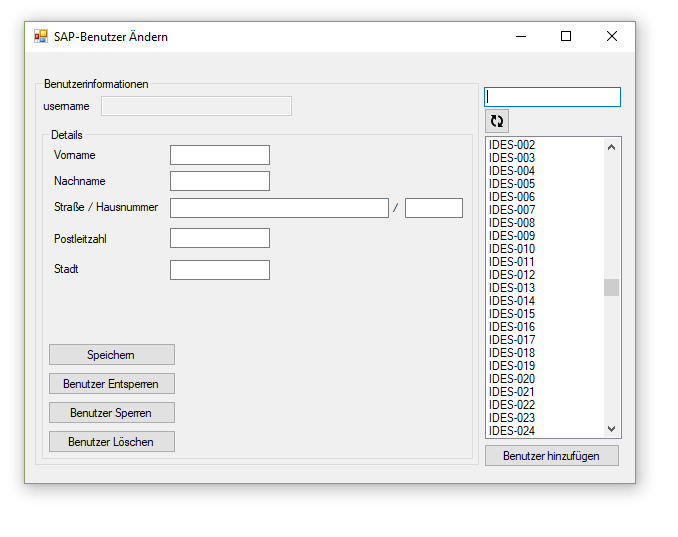
\includegraphics[width=\textwidth]{images/Main.png}
	\caption{Hauptmaske}
\end{figure}

\subsection{User-Details anzeigen}

\subsection{User erstellen}

\subsection{User editieren}

\subsection{User sperren}

\subsection{User entsperren}

\subsection{User löschen}